%!TEX root = main.tex
% \section{Data}
\subsection{Data Collection\label{sec:data}}
We collected crowdsourced segmentation data 
from Amazon Mechanical Turk where each 
HIT consisted of one segmentation task 
for a specific pre-labeled object in the image. 
There were a total of 46 objects in 9 images from the MSCOCO dataset~\cite{Lin2014}. For each object, we collected segmentation masks from a total of 40 workers.  Each worker was paid 5 cents per annotation. After eliminating segmentation masks that contains self-intersecting polygon contours, our final dataset contains 1784 bounding boxes made by 198 unique workers. As shown in Fig.\ref{interface}, each task contains a semantic keyword and a pointer indicating the object to be segmented. These tasks represent a diverse set of task difficulty (different levels of clutteredness, occlusion, lighting) and levels of task ambiguity. 
\begin{figure}[ht!]
\centering
\fbox{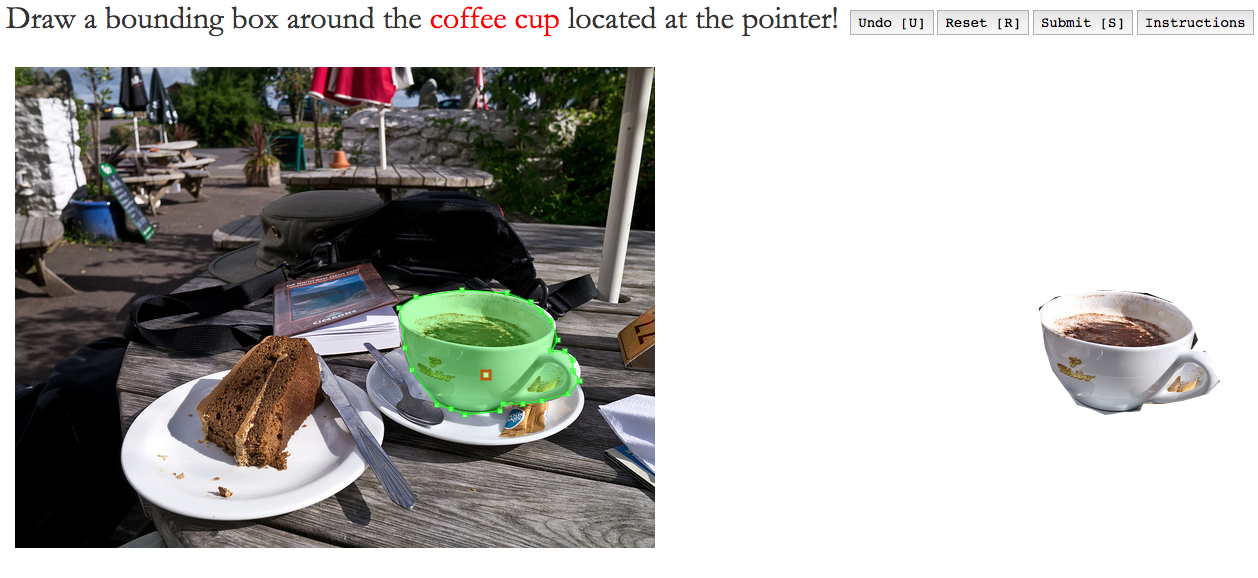
\includegraphics[width=0.9\linewidth]{plots/interface.png}}
\caption{An example interface for the segmentation webapp can be seen  \href{http://crowd-segment.herokuapp.com/segment/COCO_train2014_000000000127/10/}{here}.}
\label{interface}
\end{figure}
% We eliminated all bounding boxes \agp{likewise} from workers that were self-intersecting\agp{not clear}. 

\subsection{Worker Error patterns\label{sec:errors}}
\par Raw data collected from crowdsourced image processing tasks are known to be noisy due to varying degrees of worker skills, attention, and motivation~\cite{bell14intrinsic,MDWWelinder2010}. The average precision, recall and Jaccard similarity of the worker segmentation against the ground truth across all of the objects was 92\%, 94\%, 86\% respectively. While workers have equal rates of overbounding or underbounding behavior, workers tend to overbound by a larger amount (7212 pixels on average) than underbound (1306 pixels on average). %The distributions of worker's bounding box qualities approximately follows a transformed Gaussian (Johnson SU) distribution that accounts for the right-skewed, long-tail characteristics of the distribution\agp{this comes out of nowhere; also simplify}.
\par Visual examination of worker bounding boxes reveals several common error patterns evident across different objects. As shown in the example in Figure \ref{error_examples}, common worker errors can be classified into three types:
\begin{enumerate}
	\item \textbf{Semantic error:} Workers annotate the wrong semantic object.
	\item \textbf{Regional semantic ambiguity:}Workers annotate the correct semantic object, but included a portion connected to that object that should not have been included as part of the annotation.
	\item \textbf{Boundary imprecision:} Workers annotate the correct semantic object, but segmentation boundaries are imprecise. %(obj 17) \agp{where did obj 7 come from? point to image}
\end{enumerate}
Type 1 and 2 errors have also been observed in prior work~\cite{Sorokin2008,Lin2014,Gurari2018}, which noted that disagreement in worker responses can come from questions that are ambiguous or difficult to answer, such as segmenting a individual person from a crowd. Since there are multiple workers annotating each object, each object can suffer from multiple types of error: we found that out of the 46 objects in our dataset, 9 objects suffer from type one error and 18 objects from type two error. Almost all objects suffer from some form of type three error of varying degree of imprecision around the object boundary. The main evaluation methods highlighted in this paper focuses on resolving the type three imprecise, ``sloppy'' bounding box errors. However, since type one and two errors are also fairly severe in contributing to the recall lost, we did not want to simply eliminate objects that suffer from these issues. We will discuss a preprocessing procedure used to address these errors in Section~\ref{sec:methods}.

\agp{after having read all this, i wonder if we want to simply move the dataset description to when the evaluation happens; here just say that we look at some example worker segmentations for some tasks that we issued and try to identify general principles that can motivate the design of the algorithms, described next.}\dor{No, I agree that this would help highlight these observation as one of our contribution, this section needs to appear early on, to motivate why we have developed certain algos for resolving perspectives (e.g. clustering)}